\documentclass{beamer} %[handout]
\usetheme{CambridgeUS}
\usecolortheme{whale}
\usepackage{color}
\usepackage{xcolor}
\usepackage[makeroom]{cancel}
\usepackage{graphicx} 
\setbeamercolor{frametitle}{fg=black}
\usepackage{mathtools}
\usepackage{amssymb}
\usepackage{amsmath}
\usepackage{amsthm}
\usepackage{graphicx}
\usepackage{fancyvrb}
\usepackage{listings}
\usepackage{tikz}
\usepackage[utf8]{inputenc}

\usetikzlibrary{shapes}

\usetikzlibrary{decorations.text}

\lstset{frame=tb,
  language=R,
  aboveskip=3mm,
  belowskip=3mm,
  showstringspaces=false,
  columns=flexible,
  basicstyle={\tiny\ttfamily},
  numbers=none,
  numberstyle=\tiny\color{gray},
%  keywordstyle=\color{blue},
%  identifierstyle=\color{yellow},
  breaklines=true,
    literate={->}{$\rightarrow$}{2}
           {°}{$\epsilon$}{1},
  breakatwhitespace=true
  tabsize=3
}

\usetikzlibrary{arrows,positioning} 
\tikzset{
    %Define standard arrow tip
    >=stealth',
    %Define style for boxes
    punkt/.style={
           rectangle,
           rounded corners,
           draw=black, very thick,
           text width=6.5em,
           minimum height=2em,
           text centered},
    % Define arrow style
    pil/.style={
           ->,
           thick,
           shorten <=2pt,
           shorten >=2pt,}
}

\makeatletter
\def\th@mystyle{%
    \normalfont % body font
    \setbeamercolor{block title example}{bg=orange,fg=white}
    \setbeamercolor{block body example}{bg=orange!20,fg=black}
    \def\inserttheoremblockenv{exampleblock}
  }
\makeatother
\theoremstyle{mystyle}
\newtheorem*{remark}{Example}

\makeatletter
\def\th@mystylet{%
    \normalfont % body font
    \setbeamercolor{block title example}{bg=purple,fg=white}
    \setbeamercolor{block body example}{bg=purple!20,fg=black}
    \def\inserttheoremblockenv{exampleblock}
  }
\makeatother
\theoremstyle{mystylet}
\newtheorem*{analysis}{Example}

\date{}
\author[Bayesian statistics]{Erik \v{S}trumbelj\\2019}

\linespread{1.2}
\renewcommand{\thefootnote}{\roman{footnote}}
%\setbeameroption{show notes}

\title[Course introduction]{Course introduction}

\begin{document}

\begin{frame}

\begin{columns}[c]
\column{2in}

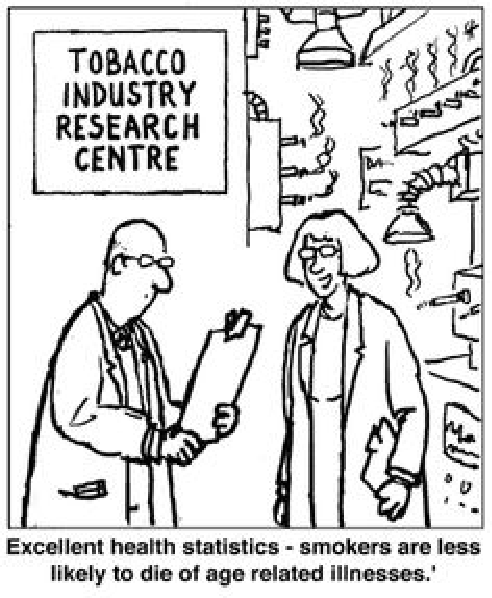
\includegraphics[width=0.90\linewidth]{../LectureAssets/L00/Lecture00cartoon}

\column{2in}
\begin{small}

\noindent \emph{\textbf{statistics}} (def.): 

\bigskip

(1) a branch of mathematics dealing with the collection, analysis, interpretation, and presentation of masses of numerical data,

\smallskip

(2)  the only science in which two recognized experts, using exactly the same set of data, may come to completely opposite conclusions.
\end{small}

\end{columns}

\bigskip

\end{frame}

\begin{frame}
Bayesian statistics
\titlepage
\end{frame}

\begin{frame}{Why Bayesian?}

\begin{itemize}\itemsep1.2em

\item Computationally intensive but conceptually simple.

\item More flexible modelling.

\item Straightforward decision-making, less prone to misinterpretation.

\item Very important in machine learning, growing presence in other fields.

\end{itemize}
\end{frame}


\begin{frame}{Course objectives}

\begin{LARGE}
\textbf{Main:} To apply Bayesian statistics in practice.
\end{LARGE}

\bigskip

\begin{itemize}\itemsep1.2em

\item Learn about the Bayesian view on probability and inference.

\item Start using tools for Bayesian statistics.

\item Understand the principles of Markov Chain Monte Carlo and their implications for Bayesian computation.

\end{itemize}

\bigskip

\end{frame}

\begin{frame}{Illustrative examples}

\bigskip

\begin{center}
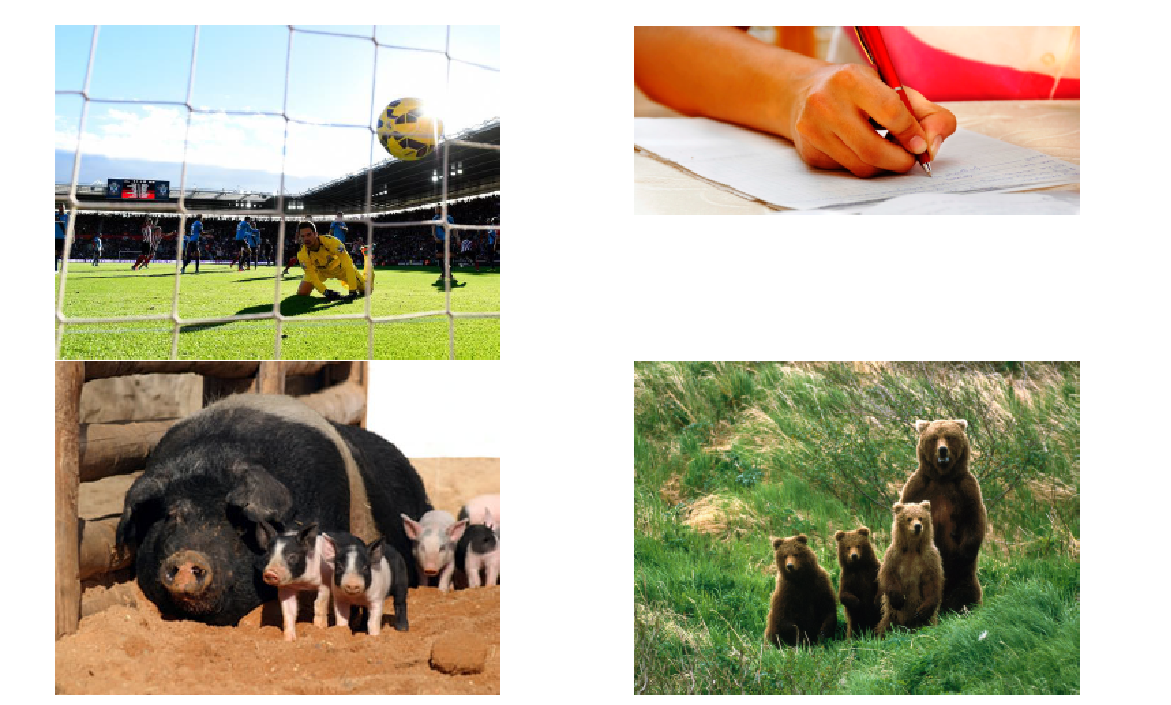
\includegraphics[width=0.80\linewidth]{../LectureAssets/L00/IllustrativeExamples}

\end{center}

\bigskip

\end{frame}

\begin{frame}[fragile]{Course information}

\textbf{Prerequisites:} Basic probability theory, basic statistics, R programming.

\bigskip

\textbf{Organization:} 8 lectures + 2 hands-on sessions.

\bigskip

\textbf{Requirements:}

\begin{itemize}
\item Take-home exercise (after first 4 lectures),
\item Final project (deadline: before end of the school year).
\end{itemize}

\bigskip

\textbf{Materials:}

\begin{itemize}
\item All slides will be made available,
\item including all code and data to reproduce what you see on the slides.
\item Further reading references will be included at end of each lecture.
\end{itemize}

\bigskip

\end{frame}

\begin{frame}{The tools that you will see me use}

Software:
\begin{itemize}
\item \textbf{R} + \textbf{RStudio},
\item \textbf{ggplot2} package for visualization,
\item \textbf{Stan} for Bayesian inference.
\end{itemize}

\bigskip

Reporting:

\begin{itemize}
\item \textbf{LaTeX} + \textbf{Texmaker},
\item \textbf{RStudio} + dynamic reports (\textbf{sweave}, \textbf{R markdown}, \textbf{R notebooks}).
\end{itemize}

\end{frame}


\begin{frame}{The Bayesian statistics timeline}
\begin{center}
\includegraphics[width=0.99\linewidth]{../LectureAssets/L00/timeline}
\end{center}
\end{frame}

\begin{frame}{Lectures outline}

\begin{enumerate}

\item \textbf{Probabilistic thinking}

\item Principles of Bayesian inference

\item Probabilistic programming with Stan

\item Estimation, group comparison and linear regression

\smallskip

------------------------ break ---------------------------

\item A gentle introduction to Markov Chain Monte Carlo

\item Hands-on session 1

\item Hierarchical modelling

\item Hands-on session 2 \& Where to go from here
\end{enumerate}
\end{frame}

\end{document}
